\documentclass{beamer}
\usepackage{graphicx}
\usepackage{../tema}


\title{Q\&A Bozzetti}
\author[C. Libralato]{C. Libralato}
\setDate{30/03/2026}

\begin{document}

{
\setbeamertemplate{footline}{}
\begin{frame}
    \titlepage
\end{frame}
}

\begin{frame}{Dashboard}
    \begin{figure}
    \centering
    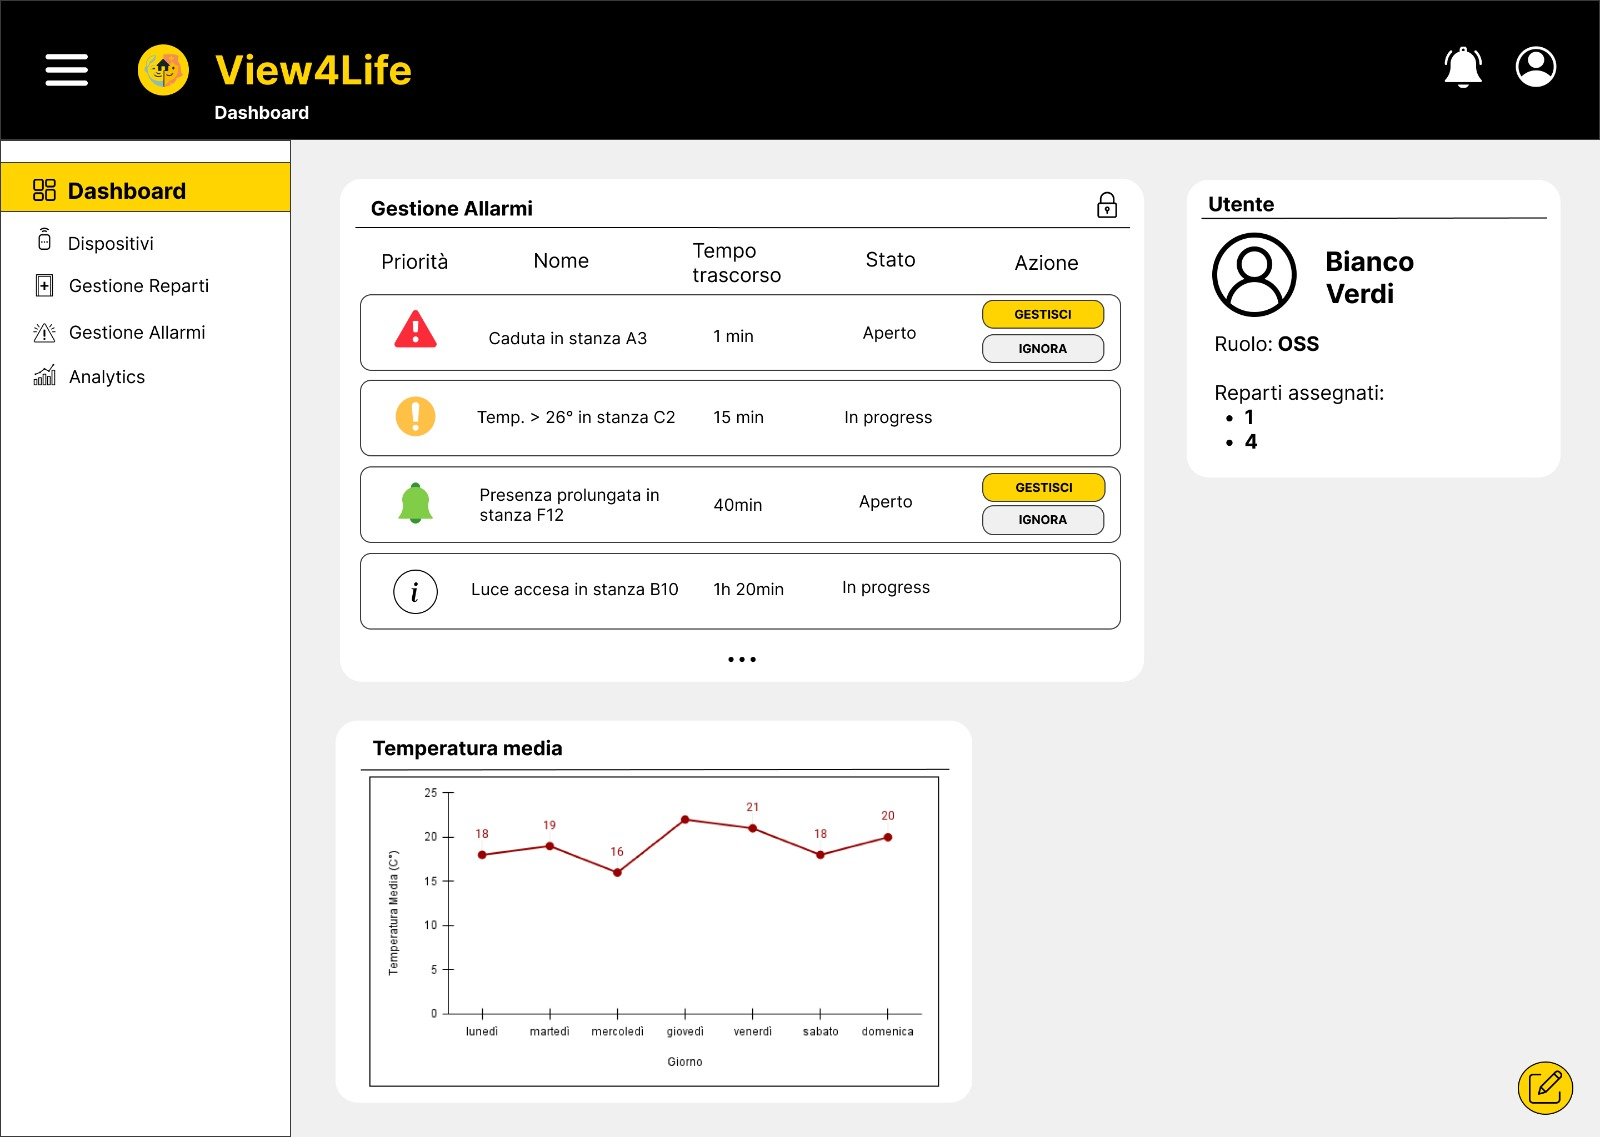
\includegraphics[
      width=\textwidth,
      height=0.5\textheight,
      keepaspectratio
    ]{dashboard.jpg}
  \end{figure}
    \begin{itemize}
        \setlength{\itemsep}{0.9em}
        \item Che caratteristiche è bene tenere a mente per trovare una disposizione che eviti click involontari?
        \item Cosa si intende con la separazione visiva delle aree con widget fissi e personalizzabili?
    \end{itemize}
\end{frame}

\begin{frame}{Dispositivi}
        \begin{figure}
    \centering
    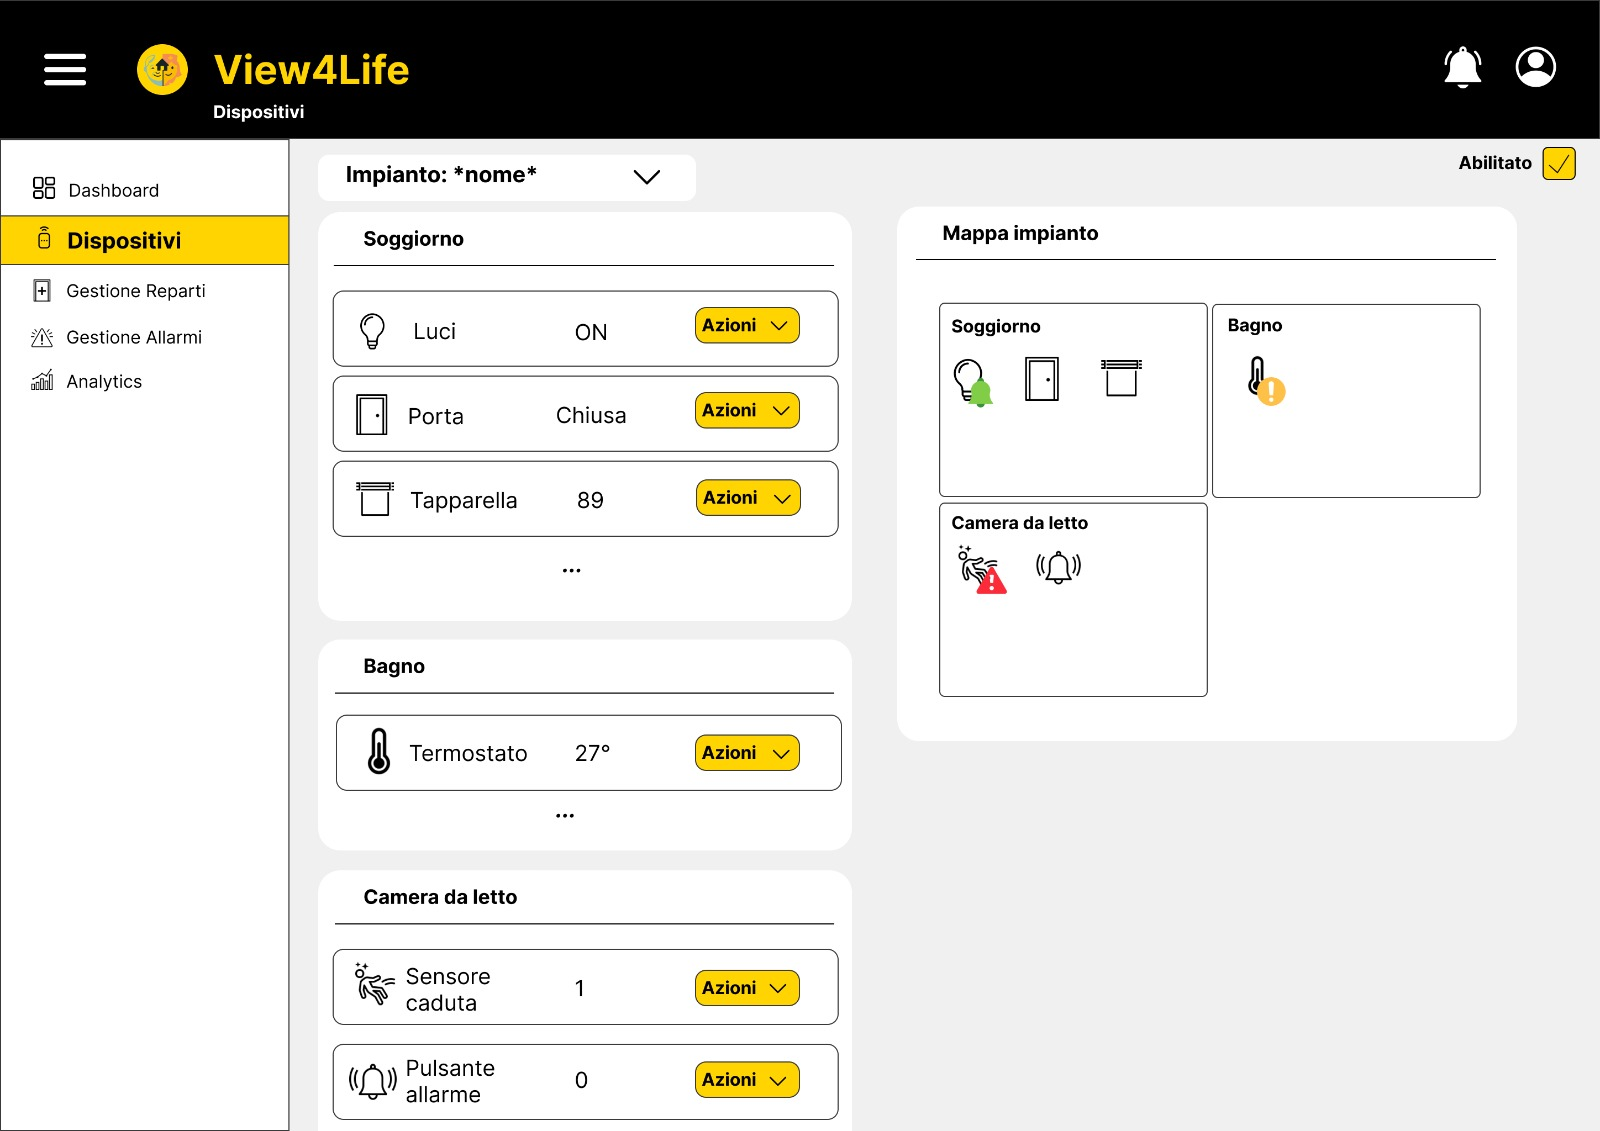
\includegraphics[
      width=\textwidth,
      height=0.5\textheight,
      keepaspectratio
    ]{devices.jpg}
  \end{figure}
    \begin{itemize}
        \setlength{\itemsep}{0.9em}
        \item Se la mappa è intesa come aiuto visuale della lista piuttosto che come suo sostituto, conviene ancora separarle?
        \item Mostrare dispositivi e allarmi disposti a matrice piuttosto che a elenco potrebbe essere valutabile?
        \item Disposizione menu di selezione impianto da chiarire.
    \end{itemize}
\end{frame}

\begin{frame}{Gestione allarmi}
     \begin{figure}
    \centering
    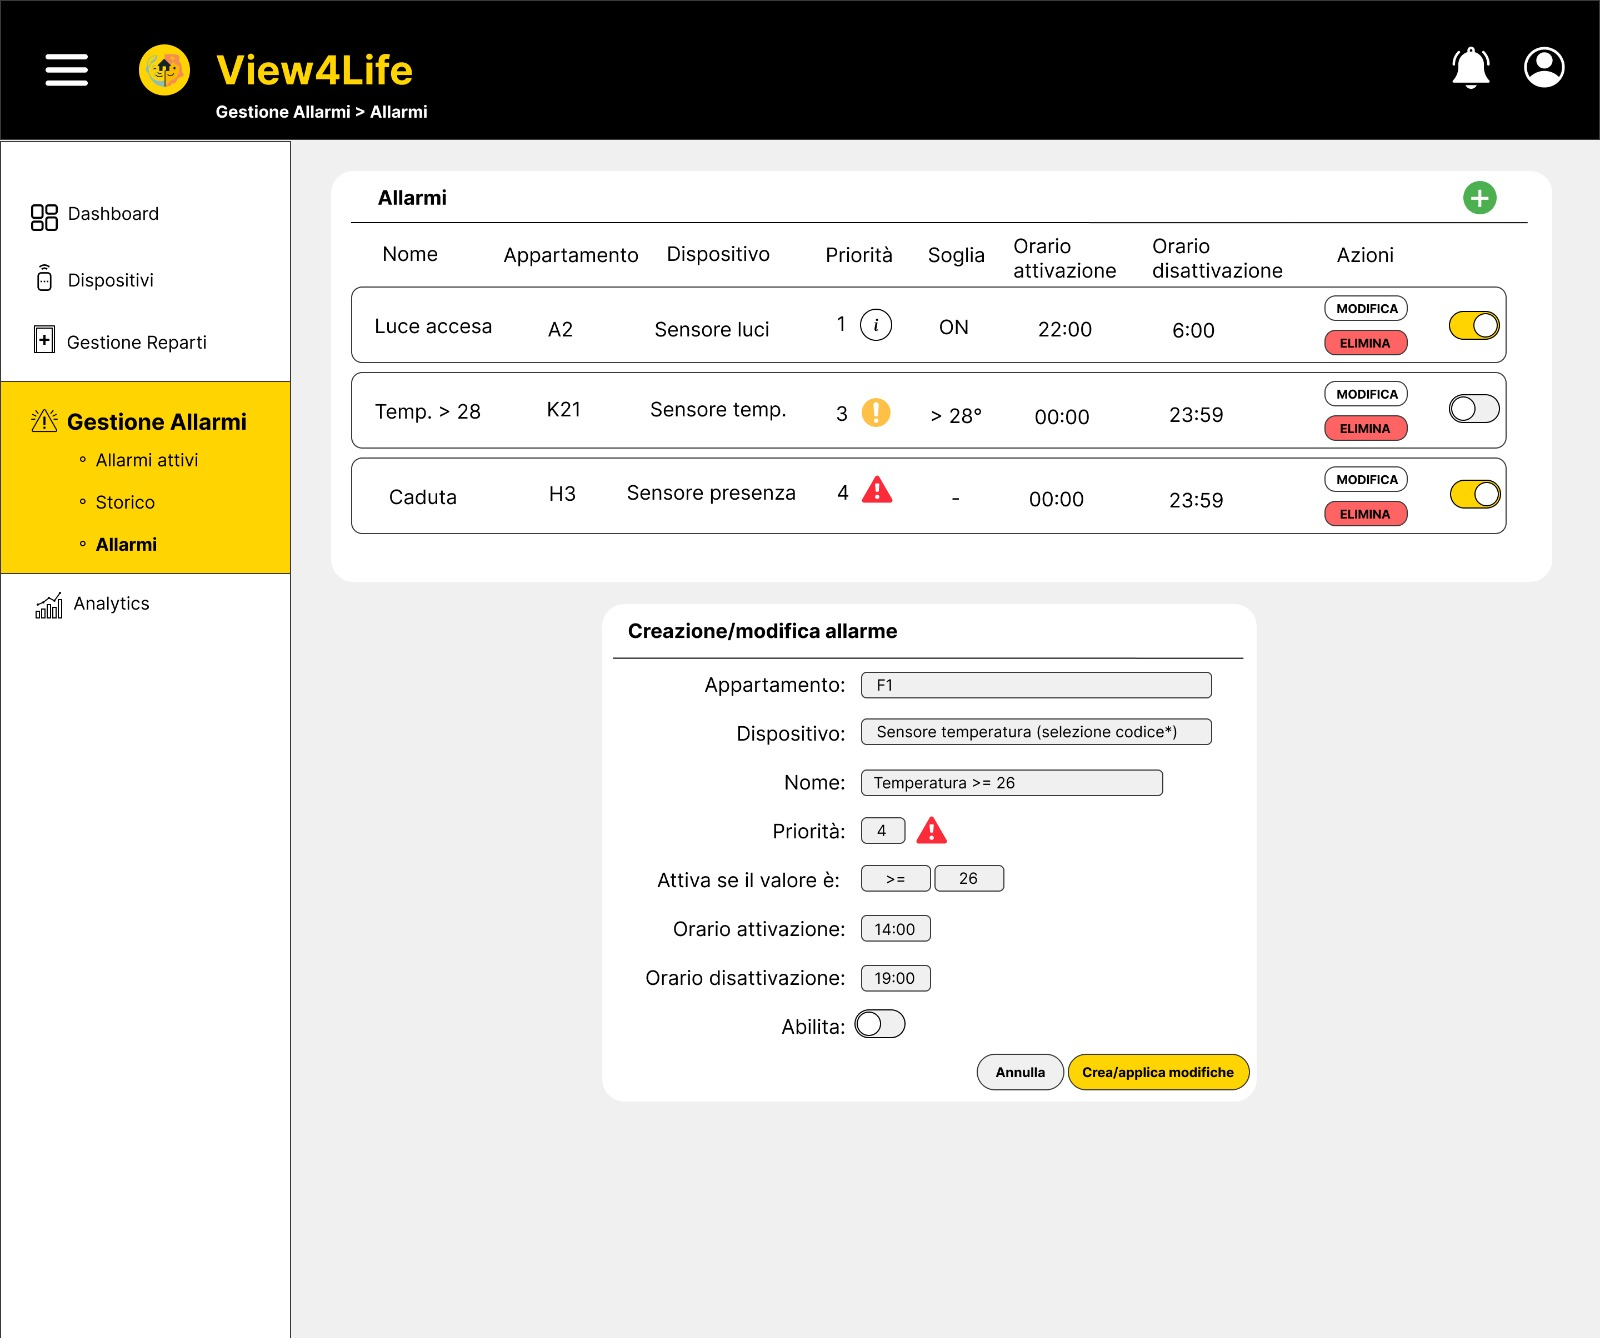
\includegraphics[
      width=\textwidth,
      height=0.5\textheight,
      keepaspectratio
    ]{alarms.jpg}
  \end{figure}
    \begin{itemize}
        \setlength{\itemsep}{0.9em}
        \item Sostituire le scritte nei bottoni con icone migliorerebbe l'estetica e l'usabilità ma rischierebbe di creare ambiguità?
        \item Per il livello di priorità degli allarmi è possibile fare affidamento esclusivamente sul colore o c'è il rischio che sia poco chiaro?        
        \item Chiarimento fraintendibilità del colore verde.
    \end{itemize}
\end{frame}

\end{document}
